\section{Bottomonia production in p+p collisions: Experimental overview}
\label{Sec:BottPP}
%In this section, we will give an overview of measurements of $\Upsilon$
%production in p+p collisions at LHC and p$\overline{\rm p}$ collisions at Tevatron. 

%% Upsilon discovery
The $\Upsilon$ meson was discovered by E288 collaboration at Fermilab in the collision of
a beam of 400 GeV protons with nucleus in 1977~\cite{PhysRevLett.39.252}.
%%Upsilon measurements at Tevatron
Detailed measurements of all the states of $\Upsilon$ were also done at Fermilab.
The Collider Detector at Fermilab (CDF) measured $\Upsilon$(1S), $\Upsilon$(2S) and $\Upsilon$(3S) 
differential ($d^{2}\sigma/dp_{T}dy$) and integrated cross sections in p$\overline{\rm p}$
collisions at $\surd s$ = 1.8 TeV~\cite{CDF:1995gwi} at Tevatron.
The three states were reconstructed via their decays 
to $\mu^{+}$ and $\mu^{-}$. The differential ($d^{2}\sigma/dp_{T}dy$) and integrated
cross sections have been measured for  $\Upsilon$(1S) in the transverse momentum range
0$\textless p_{T} \textless$16 GeV/c and for $\Upsilon$(2S) and $\Upsilon$(3S)
in the range 0$\textless p_{T}\textless$10 GeV/c.
  In 2002, CDF measured both the cross sections and polarizations of $\Upsilon$
for $|y|\textless$ 0.4 in p$\overline{\rm p}$ collisions at $\surd s$ = 1.8 TeV with
an integrated luminosity of 77 pb$^{-1}$~\cite{CDF:2001fdy} and the cross sections are
listed in Table~\ref{Tab:YCrossCDF02}. These studies helped to understand the
relative production of $\Upsilon$ states in hadronic collisions. 



%\begin{table}
%  \begin{center}
%    \caption[]{$\Upsilon$ cross sections in $|y|\textless$ 0.4 in p$\overline{\rm p}$
%      collisions at $\surd s$ = 1.8 TeV measured by CDF Run I with 
%      luminosity of 16.6 pb$^{-1}$ ~\cite{CDF:1995gwi}.}
%\label{Tab:YCrossCDF95}
%\begin{tabular}{cc} 
%\hline 
%\hline
%$\Upsilon$(nS) state             &$\frac{d\sigma(\Upsilon(nS))}{dy}\times B(\Upsilon(nS)\rightarrow\mu^{+}\mu^{-})$ (pb)    \\              
%\hline
%$\Upsilon$(1S)                   &753$\pm$29(stat.)$\pm$72(syst.)\\
%$\Upsilon$(2S)                   &183$\pm$18(stat.)$\pm$24(syst.)\\
%$\Upsilon$(3S)                   &101$\pm$15(stat.)$\pm$13(syst.)\\   
%\hline
%\hline
%\end{tabular}
%\end{center}
%\end{table}


\begin{table}
  \begin{center}
    \caption[]{The cross section of $\Upsilon$(nS) at midrapidity
($|y|\textless$ 0.4) in p$\overline{\rm p}$ collisions at $\surd s$ = 1.8 TeV with
an integrated luminosity of 77 pb$^{-1}$ as measured by CDF~\cite{CDF:2001fdy}}
\label{Tab:YCrossCDF02}
\begin{tabular}{cl} 
\hline 
\hline
$\Upsilon$(nS) state             &$\frac{d\sigma(\Upsilon(nS))}{dy}\times B(\Upsilon(nS)\rightarrow\mu^{+}\mu^{-})$ (pb)    \\              
\hline
$\Upsilon$(1S)                   &680$\pm$15(stat.)$\pm$18(syst.)$\pm$26(lumi.)\\
$\Upsilon$(2S)                   &175$\pm$9(stat.)$\pm$8(syst.)\\
$\Upsilon$(3S)                   &97$\pm$8(stat.)$\pm$5(syst.)\\   
\hline
\hline
\end{tabular}
\end{center}
\end{table}

The Run II of Tevatron was carried out at p$\overline{\rm p}$ collisions at
$\surd s$ = 1.96 TeV, and D0 experiment published results from these
experiments.
D0 experiment measured $\Upsilon$(1S) cross section in different 
rapidity ranges in p$\overline{\rm p}$ collisions at $\surd s$  = 1.96 TeV 
at luminosity of 185 pb$^{-1}$~\cite{D0:2005klj}.
Table~\ref{Tab:YCrossD0RunII} summarizes the D0 $\Upsilon$ cross section
measurements.


\begin{table}
 \begin{center}
   \caption[]{ $\Upsilon$(1S) cross sections in different rapidity ranges in p$\overline{\rm p}$
     collisions at $\surd s$ = 1.96 TeV measured in Tevatron Run II with an integrated luminosity
     of 185 pb$^{-1}$~\cite{D0:2005klj}. }
\label{Tab:YCrossD0RunII}
\begin{tabular}{cc} 
\hline 
\hline
rapidity range             &$\frac{d\sigma(\Upsilon(1S))}{dy}\times B(\Upsilon(nS)\rightarrow\mu^{+}\mu^{-})$ (pb)    \\              
\hline
0.0-0.6                   &628$\pm$16(stat.)$\pm$63(syst.)$\pm$38(lumi.)\\
0.6-1.2                   &654$\pm$17(stat.)$\pm$65(syst.)$\pm$40(lumi.)\\
1.2-1.8                   &515$\pm$16(stat.)$\pm$46(syst.)$\pm$31(lumi.)\\
0.0-1.8                   &597$\pm$12(stat.)$\pm$58(syst.)$\pm$36(lumi.)\\
\hline
\hline
\end{tabular}
\end{center}
\end{table}

The measurements of the production of $\Upsilon$(1S,2S,3S) in p+p collisions at the
unprecedented center of mass energies of 2.76, 5.02, 7, 8, and 13 TeV have been undertaken,
within various rapidity windows and in the dimuon momentum range of
$p_{T}<$ 100 GeV/c at LHC by
ATLAS~\cite{ATLAS:2011nal,ATLAS:2012lmu},
CMS~\cite{CMS:2013qur,CMS:2017dju} and LHCb collaborations \cite{LHCb:2018yzj}.

 The Large Hadron Collider (LHC) performed $\Upsilon$ measurements at 
$\surd s$ = 7 TeV in p+p collisions that is roughly four times of the Tevatron energy. 
CMS measured the $\Upsilon$ cross section in 2011 in the kinematic range 
$|y|\textless$ 2, and $p_{T} \textless$ 30 GeV~\cite{CMS:2010wld} 
with an integrated luminosity of 3.1 pb$^{-1}$.
% Table~\ref{Tab:CMSYCross7TeV} shows the CMS measurement of $\Upsilon$ cross-section.
  In 2013, CMS measured the $\Upsilon$ cross section in p+p collisions at $\surd s$ =7 TeV
with the increased integrated luminosity of 35.8 pb$^{-1}$ and in the kinematic range
$|y|\textless$ 2.4 and $p_{T}\textless$ 50 GeV~\cite{CMS:2015xqv} as shown in
Table~\ref{Tab:CMSYCrossPLB}.


%\begin{table}
%  \begin{center}
%    \caption[]{$\Upsilon$(nS) cross sections
%  in kinematic range $|y|\textless$ 2.0 and $p_{T}\textless$ 30 GeV 
%      measured by CMS in p+p collisions at $\surd s$ =7 TeV
%  for luminosity of 3.1 pb$^{-1}$~\cite{CMS:2010wld}.}
%\label{Tab:CMSYCross7TeV}
%\begin{tabular}{cl} 
%\hline 
%\hline
%$\Upsilon$(nS) state             &$ \sigma(p+p \rightarrow \Upsilon(nS)X) \times B(\Upsilon(nS)\rightarrow\mu^{+}\mu^{-})$ (nb)    \\              
%\hline
%$\Upsilon$(1S)                   &7.37$\pm$0.13(stat.)$^{+0.61}_{-0.42}$(syst.)$\pm$0.81(lumi.)\\
%$\Upsilon$(2S)                   &1.90$\pm$0.09(stat.)$^{+0.20}_{-0.14}$(syst.)$\pm$0.24(lumi.)\\
%$\Upsilon$(3S)                   &1.02$\pm$0.07(stat.)$^{+0.11}_{-0.08}$(syst.)$\pm$0.11(lumi.)\\
%\hline
%\hline
%\end{tabular}
%\end{center}
%\end{table}




\begin{table}
  \begin{center}
    \caption[]{ $\Upsilon$(nS) cross sections
  in kinematic range $|y|\textless$ 2.0 and $p_{T}\textless$ 50 GeV 
      measured by CMS in p+p collisions at $\surd s$ =7 TeV.
  for integrated luminosity of 35.8 pb$^{-1}$~\cite{CMS:2015xqv}.}
\label{Tab:CMSYCrossPLB}
\begin{tabular}{cl} 
\hline 
\hline
$\Upsilon$(nS) state             &$ \sigma(p+p \rightarrow \Upsilon(nS)X) \times B(\Upsilon(nS)\rightarrow\mu^{+}\mu^{-})$ (nb)    \\              
\hline
$\Upsilon$(1S)                   &8.55$\pm$0.05(stat.)$^{+0.56}_{-0.50}$(syst.)$\pm$0.34(lumi.)\\
$\Upsilon$(2S)                   &2.21$\pm$0.03(stat.)$^{+0.16}_{-0.14}$(syst.)$\pm$0.09(lumi.)\\
$\Upsilon$(3S)                   &1.11$\pm$0.02(stat.)$^{+0.10}_{-0.08}$(syst.)$\pm$0.04(lumi.)\\
\hline
\hline
\end{tabular}
\end{center}
\end{table}


The ATLAS experiment measured the $\Upsilon$(nS) production cross section
in p+p collisions at $\surd s$ =7 TeV in kinematic range $|y|\textless$ 2.25,
and $p_{T}\textless$ 70 GeV~\cite{ATLAS:2012lmu}.  
The results are shown in Table~\ref{Tab:ATLASYCross}.


\begin{table}
  \begin{center}
    \caption[]{ATLAS measurement of $\Upsilon$(nS) cross section in $|y|\textless$ 2.25 and $p_{T}\textless$ 70 GeV
      at $\surd s$ =7 TeV~\cite{ATLAS:2012lmu}.}
\label{Tab:ATLASYCross}
\begin{tabular}{cl} 
\hline 
\hline
$\Upsilon$(nS) state             &$ \sigma(p+p \rightarrow \Upsilon(nS)X) \times B(\Upsilon(nS)\rightarrow\mu^{+}\mu^{-})$ (nb)    \\              
\hline
$\Upsilon$(1S)                   &8.01$\pm$0.02(stat.)$\pm$0.36(syst.)$\pm$0.31(lumi.)\\
$\Upsilon$(2S)                   &2.05$\pm$0.01(stat.)$\pm$0.12(syst.)$\pm$0.08(lumi.)\\
$\Upsilon$(3S)                   &0.92$\pm$0.01(stat.)$\pm$0.07(syst.)$\pm$0.04(lumi.)\\
\hline
\hline
\end{tabular}
\end{center}
\end{table}

Several $\Upsilon$ polarization measurements have also been made. With a integrated luminosity
of 77 pb$^{-1}$, CDF measured the $\Upsilon$(1S) polarization in 2002 in 
p$\overline{\rm p}$ collisions at $\surd s$ =1.8 TeV in knematic range
$|y|\textless$ 0.4 and found that $\Upsilon$(1S) is mostly unpolarized~\cite{CDF:2001fdy}.
At $\surd s$  = 1.96 TeV, the D0 experiment measured the $\Upsilon$(1S) and
$\Upsilon$(2S) polarizations in 2008 in p$\overline{\rm p}$ data
with a integrated luminosity of 1.3 fb$^{-1}$~\cite{D0:2008yos}. The measurement done by D0 found
longitudinal polarization for the $\Upsilon$(1S)~\cite{D0:2008yos}.
However, these first polarization measurements were only done in one reference frame.
They were sensitive to the bias resulted due to the choice of the reference frame
and also to the acceptance of the detector. Later, measurements were done in multiple
reference frames which enabled the calculation of the frame invariant parameter to
prevent bias from the choice of the reference frame and detector acceptance.

The first full polarizations for all $\Upsilon$(nS) states were measured in 2012 by
CDF in Tevatron Run II at $\surd s$  = 1.96 TeV~\cite{CDF:2011ag}.
This CDF Run II measurement with a integrated luminosity of 6.7 fb$^{-1}$
with $|y|\textless$ 0.6 and $p_{T}\textless$ 40 GeV found no evidence for
polarized production of $\Upsilon$(nS) states~\cite{CDF:2011ag}.
CMS measured the $\Upsilon$(nS) polarization in 2003 in p+p collisions
at $\surd s$  = 7 TeV with a integrated luminosity 4.9 fb$^{-1}$~\cite{CMS:2012bpf}.
In these measurements, the angular distribution of the muons produced in
the $\Upsilon$(1S, 2S, 3S) decays was analyzed in different reference frames to determine the
polarization parameters. The CMS measurement found no evidence of large transverse or
longitudinal polarizations in the explored kinematic region~\cite{CMS:2012bpf}.
%The CMS polarization measurements found the $\Upsilon$(nS)
%to be unpolarized and suggested that this could be a result of
%including $\Upsilon$ produced in feeddown from an excited state~\cite{CMS:2012bpf}.
CMS measured the differential cross-section of $\Upsilon$(nS)
in p+p collisions at $\sqrt{s}$ = 13 TeV in central rapidities $|y|<2.4$,
as a function of transverse momentum in high momentum range~\cite{CMS:2017dju}.
These are used to constrain the theoretical calculations in the high
momentum range as shown in the next section~\ref{sec:Bottomonia_pp_th}.

The $\Upsilon$(nS) cross sections are measured by LHCb~\cite{LHCb:2018yzj}
in p+p collisions at $\sqrt{s}=13$ TeV, in transverse momentum
range $0 < pT < 15$ GeV/$c$ and forward rapidity region $2 < y < 4.5$.
The cross sections are listed here. \\
B($\Upsilon$(1S) $\rightarrow$ $\mu^+\mu^-$) $\times$ $\sigma$($\Upsilon$(1S)) = 4687 $\pm$ 10 $\pm$ 294 pb,\\
B($\Upsilon$(2S) $\rightarrow$ $\mu^+\mu^-$) $\times$ $\sigma$($\Upsilon$(2S)) = 1134 $\pm$ 6 $\pm$ 71 pb, \\
B($\Upsilon$(3S) $\rightarrow$ $\mu^+\mu^-$) $\times$ $\sigma$($\Upsilon$(3S)) = 561 $\pm$ 4 $\pm$ 36 pb. 


The measurements of the cross sections and polarizations have shed light on the
$\Upsilon$(1S, 2S, 3S) production mechanisms in p+p collisions.
LHC data has substantially extended the reach of the kinematics to test the
Non-Relativistic QCD (NRQCD) and other models with
higher-order corrections which becomes more distinguishable with the increase of $p_{T}$.


\section{Bottomonia production mechanism in p+p collisions}
\label{sec:Bottomonia_pp_th}

In general, one can subdivide the quarkonia production process into two major parts;
the production of a heavy quark pair in hard collisions and the formation of quarkonia
out of the two heavy quarks.
  The massive quarks (with $m_c\sim 1.6$ GeV/$c^2$, $m_b\sim 4.5$ GeV/$c^2$) are produced
in the initial stages of hadronic collision with high momentum transfer and 
can be treated perturbatively~\cite{Nason:1989zy}. The formation of quarkonia
from the two massive quarks is a non-perturbative phenomenon that is
described using different effective models~\cite{Bodwin:1994jh,Brambilla:2014jmp}.
The Color Singlet Model (CSM)~\cite{Einhorn:1975ua,Berger:1980ni},
Color Evaporation Model (CEM)~\cite{Fritzsch:1977ay,Amundson:1995em}, the Fragmentation
Scheme and the NRQCD factorisation formalism are some of the popular
approaches used for quarkonia production.


%Due to the high mass of the heavy quarks they are produced in the initial
%collisions as their production requires sufficiently high momentum 
%transfers. For this reason, the heavy quark (mass $m$) production
%is a hard process that can be treated perturbatively.
The hadronic cross section in $p+p$ collisions at center of mass energy
$\sqrt{s}$ can be written as
\begin{eqnarray}
\sigma_{pp}(s,m^2) & = & \sum_{i,j = q, \overline q, g} 
\int dx_1 \, dx_2 \, 
f_i^p (x_1,\mu_F^2) \,
f_j^p(x_2,\mu_F^2) \, \widehat{\sigma}_{ij}(\hat{s},m^2,\mu_F^2,\mu_R^2).
\label{sigpp}
\end{eqnarray}
Here, $f_i^p$ are the parton (${i = q, \overline q, g}$) densities of the proton,
$x_1$ and $x_2$ are the fractional momenta carried by the colliding
partons and $\mu_F$ and $\mu_R$ are, respectively, fragmentation and renormalization scales. 
The total partonic cross section has been calculated up to NLO
\cite{Nason:1989zy,Nason:1987xz} and can be expressed as
\begin{eqnarray}
\widehat{\sigma}_{ij}(\hat{s},m,\mu_F^2,\mu_R^2) & = & 
\frac{\alpha_s^2(\mu_R^2)}{m^2}
\left\{ f^{(0,0)}_{ij}(\rho) \right. \nonumber \\
 & + & \left. 4\pi \alpha_s(\mu_R^2) \left[f^{(1,0)}_{ij}(\rho) + 
f^{(1,1)}_{ij}(\rho)\ln\bigg(\frac{\mu_F^2}{m^2} \bigg) \right] 
+ {\cal O}(\alpha_s^2) \right\},
\,\, 
\label{sigpart}
\end{eqnarray}
where $\rho = 4m^2/\hat{s}$ and 
$f_{ij}^{(k,l)}$ are the scaling functions to NLO \cite{Nason:1989zy,Nason:1987xz}. 
At small $\rho$, the ${\cal O}(\alpha_s^2)$ and ${\cal O}(\alpha_s^3)$
$q \overline q$ and the ${\cal O}(\alpha_s^2)$ $gg$ scaling functions 
become small while the ${\cal O}(\alpha_s^3)$ $gg$ and $qg$ scaling functions
plateau at finite values.  Thus, at collider energies, the total cross sections
are primarily dependent on the small $x$ parton densities and phase space.
The total cross section does not depend on any kinematic variables. It depends  
only on the quark mass, $m$, and the renormalization and factorization scales with central
values $\mu_{R,F} =\mu_0 = m$.


The formation of quarkonium through a nonperturbative evolution of the $Q\bar Q$ pair 
has been discussed extensively using different models and also in the framework of the 
  effective field theories of QCD
\cite{Bodwin:1994jh,Brambilla:2004wf}. Different
treatments of this evolution have led to various theoretical models for
inclusive quarkonium production. Most notable among these are the color-singlet
model (CSM), the color-evaporation model (CEM) and the non-relativistic QCD
(NRQCD) factorization approach. In this review, we will describe CEM and NRQCD 
approaches and their results in comparison with the measurements 

\subsection{The color singlet model}

The color singlet model (CSM) was proposed shortly after the discovery of the 
J/$\psi$~\cite{Einhorn:1975ua,Berger:1980ni,Ellis:1976fj,Carlson:1976cd}.
In CSM model, it is assumed that the $Q\bar Q$ pair which evolves into
the quarkonium is in a color-singlet state and also the pair has the same spin
and angular-momentum quantum numbers as the final quarkonium.
In the CSM, the production rate for the quarkonium state is obtained in terms of 
the absolute values of the color-singlet $Q\bar Q$ wave function and its
derivatives, evaluated at zero $Q\bar Q$ separation.
These quantities can be extracted by comparing theoretical 
calculations in the CSM with experimental measurements. Once these quantities 
are extracted the CSM  can predict the cross sections at any given collision energy.
At low energies, the CSM can successfully  predict the quarkonium
production cross sections~\cite{Schuler:1994hy}.
But, at high energies, very large corrections to the CSM appear at next-to-leading
order (NLO) and next-to-next-to-leading order (NNLO) in $\alpha_s$
\cite{Artoisenet:2007xi,Campbell:2007ws,Artoisenet:2008fc}.
It thus indicates that there may be some additional production mechanism emerging at
high energy. However, given the very large corrections at
NLO and NNLO, it is not clear that the perturbative expansion in
$\alpha_s$ is convergent. 

\subsection{The color evaporation model}  
\label{prod_sec:CEM}

The CEM~\cite{Fritzsch:1977ay,Amundson:1995em,Amundson:1996qr}
is motivated by the principle of quark-hadron duality. In the CEM, it
is assumed that every produced $\QQbar$ pair can evolve into a quarkonium
if it has an invariant mass that is less than the threshold for
producing a pair of open-flavor heavy mesons. It is further assumed that
the nonperturbative probability for the $\QQbar$ pair to evolve into a
quarkonium state $H$ is given by a constant $F_H$ that is independent of 
energy-momentum and process. Once $F_H$ has been fixed by
comparison with the measured total cross section for the production of
the quarkonium $H$, the CEM has no more free parameters and
can predict, the momentum distribution of the quarkonium production rate
at any collision energy.
The CEM predictions provide good descriptions of the CDF data for $\Jpsi$,
$\psi(2S)$ and $\chi_{c}$ production at $\sqrt{s}=1.8$~TeV
\cite{Amundson:1996qr}. 


The quarkonium production cross sections are calculated in the
color evaporation model with normalizations determined by fitting the
scale parameter to the shape of the energy-dependent cross sections in Ref.~\cite{Nelson:2012bc}.
The production cross sections for heavy flavor and quarkonia at $\sqrt{s_{\rm NN}}$ = 5.02 
TeV~\cite{Kumar:2012qx} calculated using CEM are given in Table~\ref{NLOcros}.
The bottom quark production cross section is calculated to NLO in pQCD  
using the CT10 parton densities \cite{Lai:2010vv}.
The quark mass and scale parameters are $m_b = 4.65 \pm 0.09$ GeV,
$\mu_F/m_{T\, b} = 1.40^{+0.75}_{-0.47}$, and $\mu_R/m_{T\, b} = 1.10^{+0.26}_{-0.19}$.
The central EPS09 NLO parameter set~\cite{Eskola:2009uj} is used to 
calculate the modifications of the parton distribution functions (nPDF) in 
Pb+Pb collisions, referred to as cold nuclear matter (CNM) effects.
The yields in a minimum bias 
Pb+Pb event is obtained from the per nucleon cross
section, $\sigma_{\rm PbPb}$, in Table~\ref{NLOcros}, as
\begin{eqnarray}
N = {A^2 \sigma_{\rm PbPb} \over  
\sigma_{\rm PbPb}^{\rm tot}} \, \, .
\end{eqnarray}

At 5.02 TeV, the total Pb+Pb cross section, $\sigma_{\rm PbPb}^{\rm tot}$, 
is 7.7 b~\cite{Loizides:2017ack}.


%\begin{table}
%  \begin{center}
%\caption[]{Heavy quark and quarkonia production  cross sections at
%$\sqrt{s_{_{_{NN}}}}= 2.76$ TeV. The cross sections are given per nucleon pair while
%$N^{\rm PbPb}$ gives the initial number of heavy quark pair/quarkonia per Pb+Pb event.}
%\label{NLOcros}
%\begin{tabular}{l|l|l|l|l} 
%\hline 
%\hline
%             & $ c \overline c$            &$\Jpsi$                      & $ b \overline b$                    & $\Upsilon$   \\              
%\hline
%$\sigma_{pp}$ & $4.11^{+2.69}_{-2.50}$ mb    & $21.6^{+10.6}_{-10.4}~\mu$b   & $110.5^{+15.1}_{-14.2}~\mu$b            & $0.22^{+0.07}_{-0.06}~\mu$b  \\
%
%
%$\sigma_{\rm PbPb}$ & $3.21^{+2.1}_{-1.95}$ mb    &16.83$^{+8.26}_{-8.10}~\mu$b    & $100.5^{+13.7}_{-12.9}~\mu$b             & 0.199$^{+0.063}_{-0.054}~\mu$b  \\
%$N^{\rm PbPb}$     & $18.12^{+12}_{-11}$       & $0.0952^{+0.047}_{-0.046}$         & $0.57^{+0.08}_{-0.07}$                          & $0.001123^{+0.0004}_{-0.0003}$       \\
%\hline
%\hline
%\end{tabular}
%\end{center}
%\end{table}




\begin{table}
  \begin{center}
\caption[]{Heavy quark and quarkonia production  cross sections at
$\sqrt{s_{_{_{NN}}}}=$ 5.02 TeV. The cross sections are given per nucleon pair while
$N^{\rm PbPb}$ gives the initial number of heavy quark pair/quarkonia per Pb+Pb event.}
\label{NLOcros}
\begin{tabular}{l|l|l} 
\hline 
\hline
                        & $ b \overline b$                    & $\Upsilon$   \\              
\hline
$\sigma_{pp}$            & $210.3^{+70.8}_{-77.6}~\mu$b            & $0.42^{+0.14}_{-0.16}~\mu$b  \\


$\sigma_{\rm PbPb}$        & $179.3^{+60.3}_{-66.2}~\mu$b             & 0.359$^{+0.121}_{-0.132}~\mu$b  \\



$N^{\rm PbPb}$              & $1.007^{+0.339}_{-0.372}$               & $0.0020^{+0.0007}_{-0.0007}$   \\

\hline
\hline
\end{tabular}
\end{center}
\end{table}


Recently, work in Ref.~\cite{Cheung:2018upe} presents an Improved Color Evaporation Model
(ICEM). They obtained bottomonium production cross sections as a function of
transverse momentum and rapidity and calculate the polarization of prompt
$\varUpsilon$($n$S) production at leading order employing the $k_T$-factorization approach.
We reproduce here some of the representative calculations using ICEM.

Figure~\ref{CMS_1S_pt} shows the
differential cross section for $\varUpsilon$(1S) production as a function
  of $p_T$ in p+p collisions at $\sqrt{s} = 7$~TeV in midrapidity, $|y|<2.4$, calculated using
ICEM~\cite{Cheung:2018upe} with combined mass and renormalization scale
uncertainties (blue).  Also shown are the calculations with CEM using a collinear
factorization approach (magenta). The calculations are compared with the CMS
midrapidity data \cite{CMS:2013qur}.

Figure~\ref{CMS_2S_3S_pt} shows the
differential production cross sections of prompt $\varUpsilon$(2S) (left)
and prompt $\varUpsilon$(3S) (right) as a function
of $p_T$ in p+p collisions at $\sqrt{s} = 7$~TeV in midrapidity, $|y|<2.4$, 
calculated using ICEM~\cite{Cheung:2018upe} with combined mass and renormalization
scale uncertainties compared with the CMS midrapidity data \cite{CMS:2013qur}.

These results show that the $p_{\rm T}$ dependence of the cross sections of all three states
is explained by ICEM within the model uncertainties. The model gives 
probability $F_H$ for the $\QQbar$ pair to evolve into a 
quarkonium state $H$.
  
\begin{figure*}
\centering
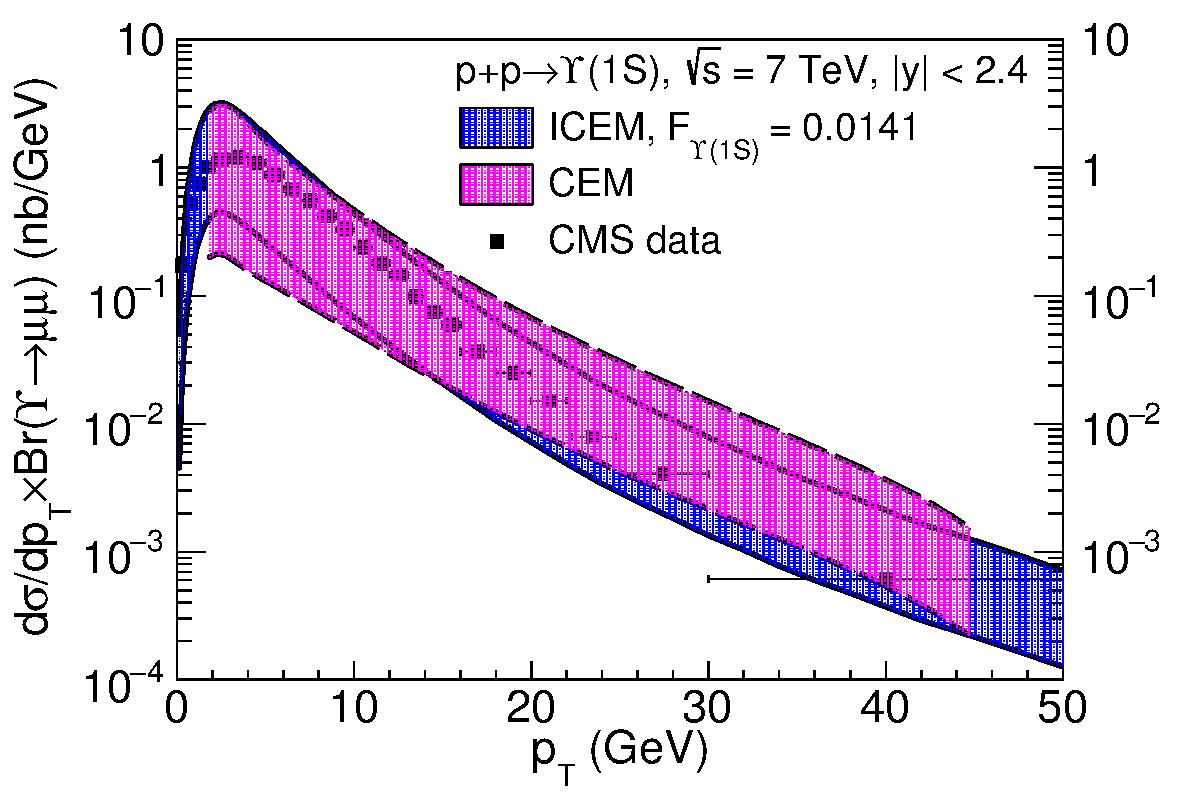
\includegraphics[width=0.60\textwidth]{Figures/Fig1_RV1S.pdf}
\caption{(Color online) The differential cross section for $\varUpsilon$(1S) production as a function
  of $p_T$ in p+p collisions at $\sqrt{s} = 7$~TeV in midrapidity $|y|<2.4$ calcuated using
ICEM~\cite{Cheung:2018upe} with combined mass and renormalization scale
uncertainties (blue).  Also shown the are calculations with CEM using collinear
factorization approach (magenta).
 The calculations are compared with the CMS midrapidity data \cite{CMS:2013qur}.}
\label{CMS_1S_pt}
\end{figure*}



\begin{figure*}
\centering
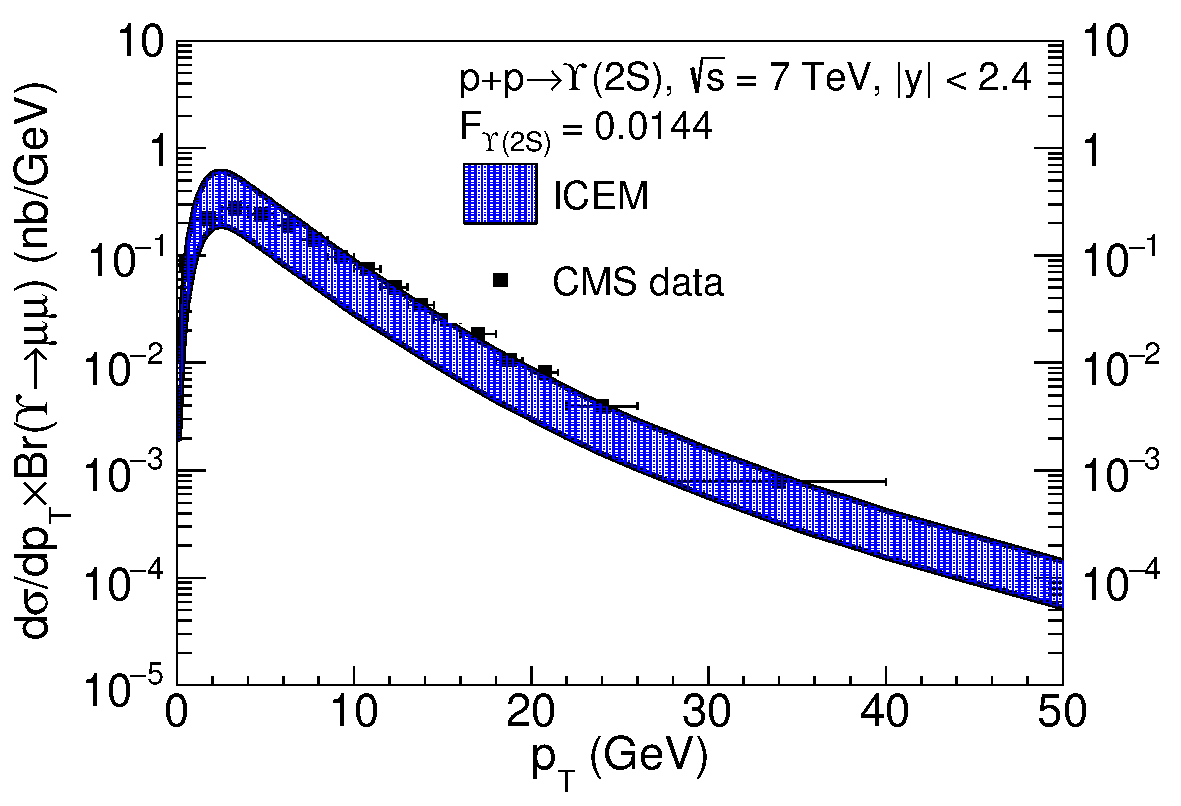
\includegraphics[width=0.48\textwidth]{Figures/Fig2l_RV2S.pdf}
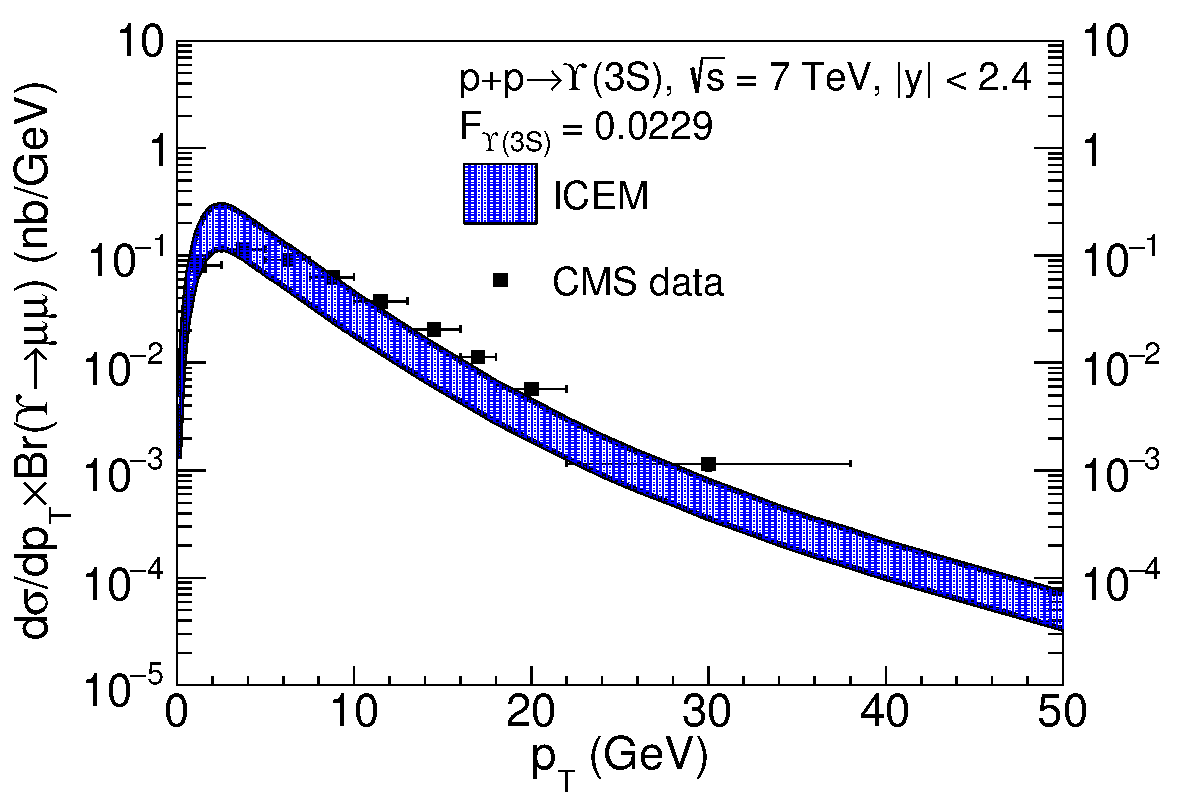
\includegraphics[width=0.48\textwidth]{Figures/Fig2r_RV3S.pdf}
\caption{(Color online) The differential production cross sections of prompt $\varUpsilon$(2S) (left)
  and prompt $\varUpsilon$(3S) (right) as a function
  of $p_T$ in p+p collisions at $\sqrt{s} = 7$~TeV in midrapidity, $|y|<2.4$
  calculated using ICEM~\cite{Cheung:2018upe} with combined mass and renormalization
  scale uncertainties compared with the CMS midrapidity data \cite{CMS:2013qur}.}
\label{CMS_2S_3S_pt}
\end{figure*}








\subsection{The NRQCD factorization approach}


The $Q\bar{Q}$ pair, evolving into the quarkonium,
is assumed to have the same spin and angular momentum same as that of quarkonium.
NRQCD approach incorporates both the color singlet as
well as the Color Octet (CO) states of quarkonium.
In the formalism of the NRQCD factorisation approach, the evolution
probability of $Q\bar{Q}$ pair into a state of quarkonium is expressed as matrix
elements of NRQCD operators.
These operators are expanded
in terms of the velocity $v$ (for $v\ll$1) of heavy quarks~\cite{Bodwin:1994jh}.
The production cross-sections and decay rates of quarkonia states are then
calculated using factorisation formulae.
The full structure of the $Q\bar{Q}$ Fock space
is spanned by $n$=$^{2s+1}L_J^{[a]}$ state where $L$ is the orbital angular momentum, $s$
is the spin, $J$ is the total angular momentum
and $a$ (color multiplicity) = 1 for CS and 8 for CO states. 
The produced CO states of $Q\bar{Q}$ pair at short distances finally emerge as 
CS quarkonia by emitting soft gluons non-perturbatively.


There have been several studies on bottomonia production based on
NRQCD formalism \cite{Domenech:1999qg,Domenech:2000ri,Braaten:2000cm,Gong:2010bk,Sharma:2012dy}.
Both the production and polarisation of $\Upsilon$(nS) at NLO have been discussed in 
Ref.~\cite{Gong:2013qka} within the framework of NRQCD.
The CO matrix elements are obtained by fitting the calculations with experimental data.
The study is updated in Ref.~\cite{Feng:2015wka} by considering
feed down from $\chi_{bJ}$(mP) states in $\Upsilon$(nS) production.
The yields and polarisations of $\Upsilon$(nS) measured at Tevatron and
LHC are well explained by this work.
The NLO study in Ref.~\cite{Han:2014kxa} includes feed down contributions
from higher states and describes the cross sections and
polarisations of $\Upsilon$(nS) at LHC energy.
In Ref.~\cite{Yu:2017pot}, production cross-section for $\Upsilon$(nS),
$\chi_{bJ}$, $\eta_b$ and $h_b$ have been calculated using NRQCD, as produced
in hard photo production and fragmentation processes at LHC energies. 
In Ref.~\cite{Kumar:2021sek} it is shown that there is a large difference among the
Long Distance Matrix Element (LDME)s obtained by different analyses at NLO.

In Ref.~\cite{Kumar:2021sek} the LO NRQCD calculations for the differential production
cross-sections of $\Upsilon$ states in p+p collisions have been discussed. 
This work uses a large set of data from Tevatron~\cite{Acosta:2001gv} and
LHC~\cite{CMS:2013qur,LHCb:2012aa,CMS:2015xqv,ATLAS:2012lmu,CMS:2017dju} 
to extract the LDMEs required for the $\Upsilon$ production.
It is to be noted that an LO NRQCD analyes is straightforward and has excellent
predictability power for unknown cross sections.

%and then results are
%presented in Section~\ref{sec:results}.
%A comparison of the obtained LDMEs with the
%previous NRQCD studies both at LO and NLO has been made.
%The summary 
%of our findings are discussed in Section~\ref{sec:summary}. An updated QCD LO study on the
%bottomonia hadroproduction is useful as it provides a reference for comparison
%with NLO calculations. 

The processes that govern the production of heavy mesons like bottomonium,
can be denoted generically by 
$i+j\rightarrow \Upsilon +X$, where $i$ and $j$ are the incident light partons,
$\Upsilon$ is the heavy meson and $X$ is final state light parton.
The double differential cross-section as a function of $p_T$ and rapidity ($y$) of 
the heavy meson can be written as~\cite{Kumar:2016ojy},
\begin{eqnarray}
  E\,\frac{d^3\sigma^{\Upsilon} }{d^3p} &=& \sum_{i,j=q,\overline{q},g} \int dx_1 dx_2 f_{i}^p(x_1,\mu_F^2)
  f_{i}^p(x_2,\mu_F^2) \delta(s+u+t-m^2) {\hat{s} \over \pi} \, \frac{d\sigma}{d\hat{t}}.
  \label{eq4}
\end{eqnarray}
where, $f_{i}^p$($f_{j}^p$) are distribution functions of the colliding parton $i(j)$ in
the incident protons as a function of $x_1$($x_2$); the fractions of the total momentum
carried by the incident partons and the scale of factorisation $\mu_F$.
Here $\sqrt{s}$ is the total center of mass energy of the p+p system and $m_T~(=\mu_F)$ stands for
the transverse mass, $m_T^2=p_T^2 + M^2$ of the quarkonium.
The ${d\sigma}/{d\hat{t}}$ in Eq.~\ref{eq4} is the parton level cross-section and is
defined as~\cite{Bodwin:1994jh},
\begin{equation}
  \frac{d\sigma}{d\hat{t}} = \frac{d\sigma}{d\hat{t}}(ab\rightarrow Q\bar{Q}(^{2s+1}L_J)+X)
  M_L(Q\bar{Q}(^{2s+1}L_J)\rightarrow \Upsilon)
  \label{eq6}
\end{equation}
The first term in RHS is the short distance contribution, which corresponds to the $Q\bar{Q}$
pair production in a specific color and spin configuration and is calculable using 
perturbative QCD (pQCD)~\cite{Braaten:2000cm,Baier:1983va,Humpert:1986cy,Gastmans:1987be,Cho:1995vh,Cho:1995ce}.
The other term in the RHS of Eq.(\ref{eq6}) is the LDME 
and gives the probability of the $Q\bar{Q}$ converting into a quarkonium state.
They are determined by comparing the calculations with the measurements.

The quarkonium yield depends on the $^3S_1^{[1]}$ 
and $^3P_J^{[1]}$(J=0,1,2) CS states and $^1S_0^{[8]}$, $^3S_1^{[8]}$ and $^3P_J^{[8]}$
CO states in the limit $v\ll 1$.
The superscripts in square brackets represent the color structure of the bound state,
1 for the CS and 8 for the CO.



\begin{figure}
  \centering
  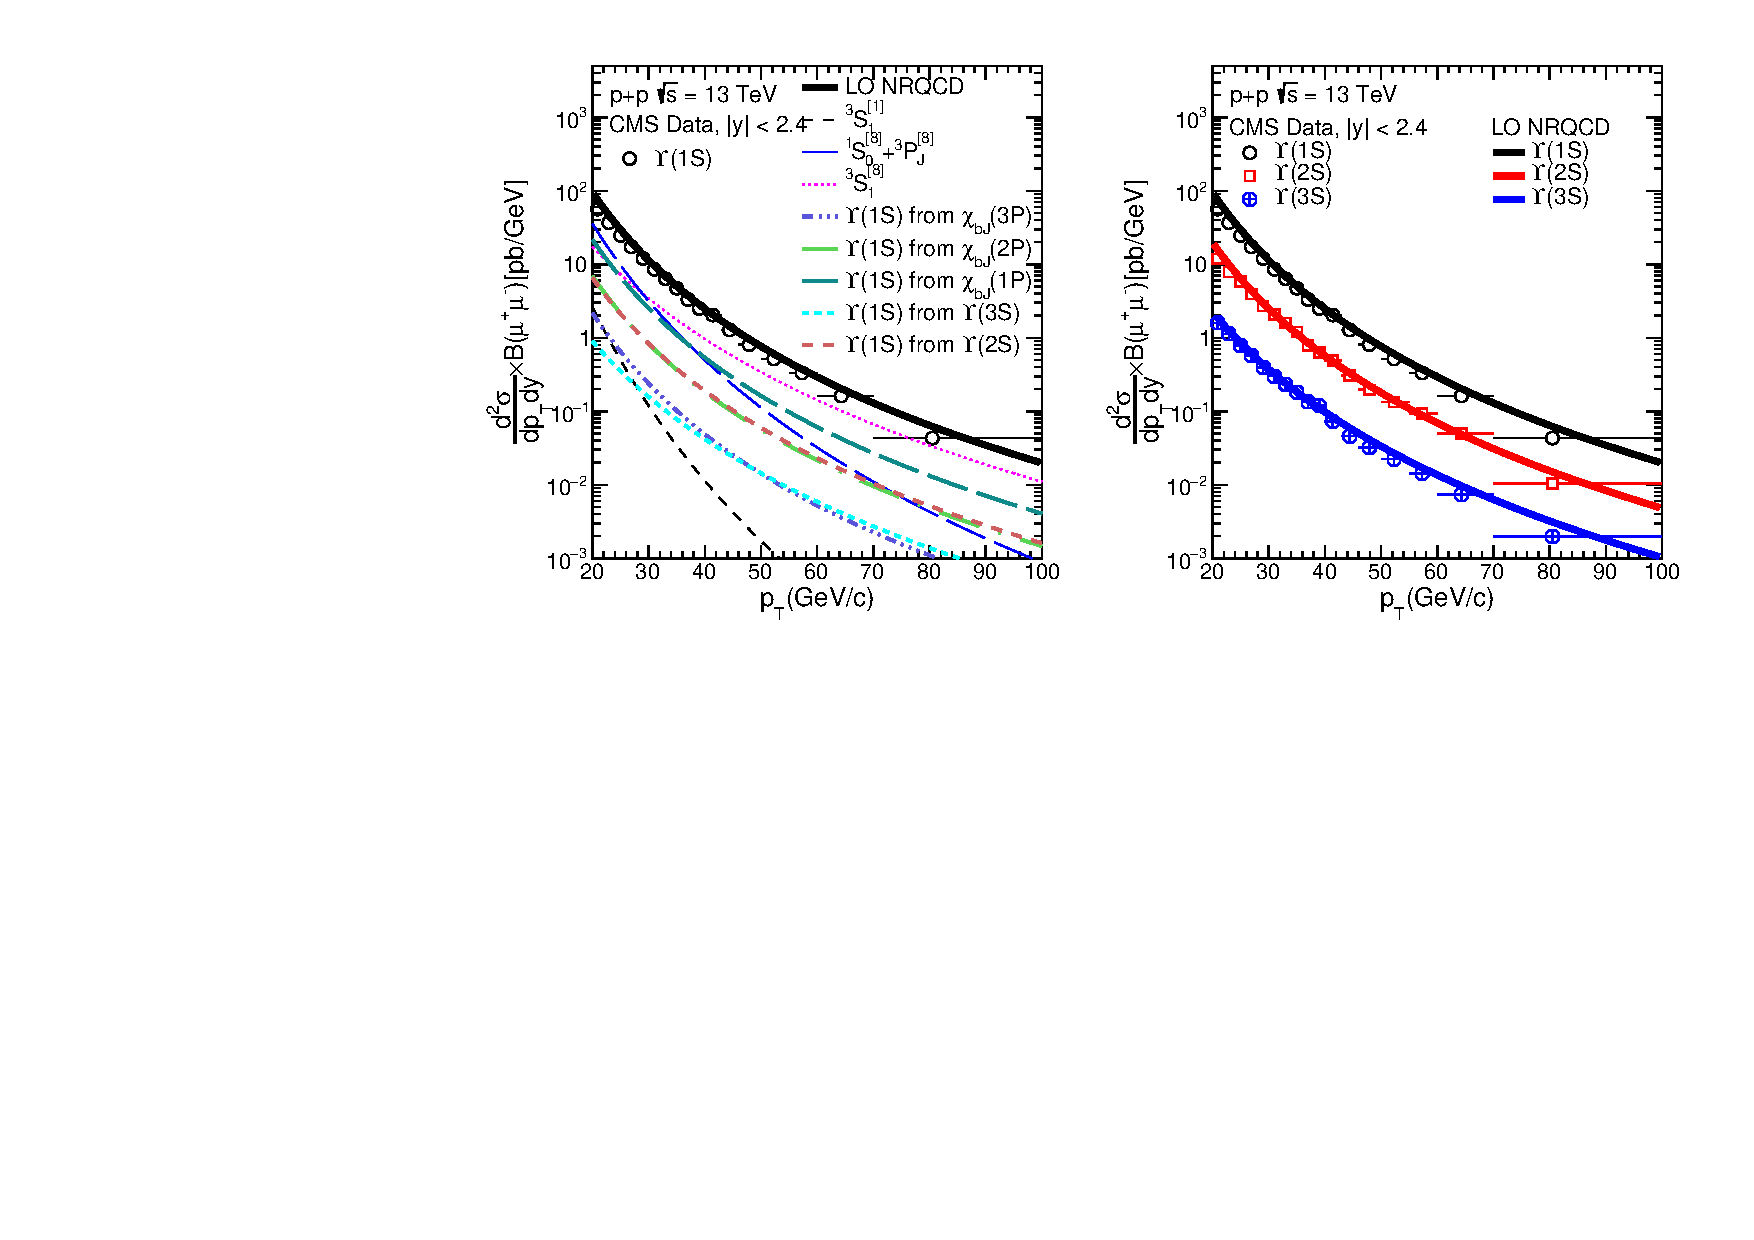
\includegraphics[width=0.99\textwidth]{Figures/Fig3_CMS_YnS_Rap12_13TeV_Pt.pdf}
  \caption{\small{(Color online) The NRQCD calculations~\cite{Kumar:2021sek} of the production cross-section of $\Upsilon$(nS)
      in p+p collisions at $\sqrt{s}$ = 13 TeV in central rapidities, as a function of
      transverse momentum, compared with the measured data at CMS~\cite{CMS:2017dju}
      experiment. The left figure shows relative contributions in $\Upsilon$(1S) from
      singlet and octet states as well as from feed down. The right figure shows the sum
      of all contributions for all the 3 states where the results for $\Upsilon$(1S) and
      $\Upsilon$(2S) are shifted vertically by factors of 10 and 5, respectively
      for better visibility.}}
  %   The LDMEs are obtained by a combined fit of the CMS and ATLAS data.}
  \label{Fig:SigmaYnSCMS13TeV}
\end{figure}



\begin{figure}
  \centering
  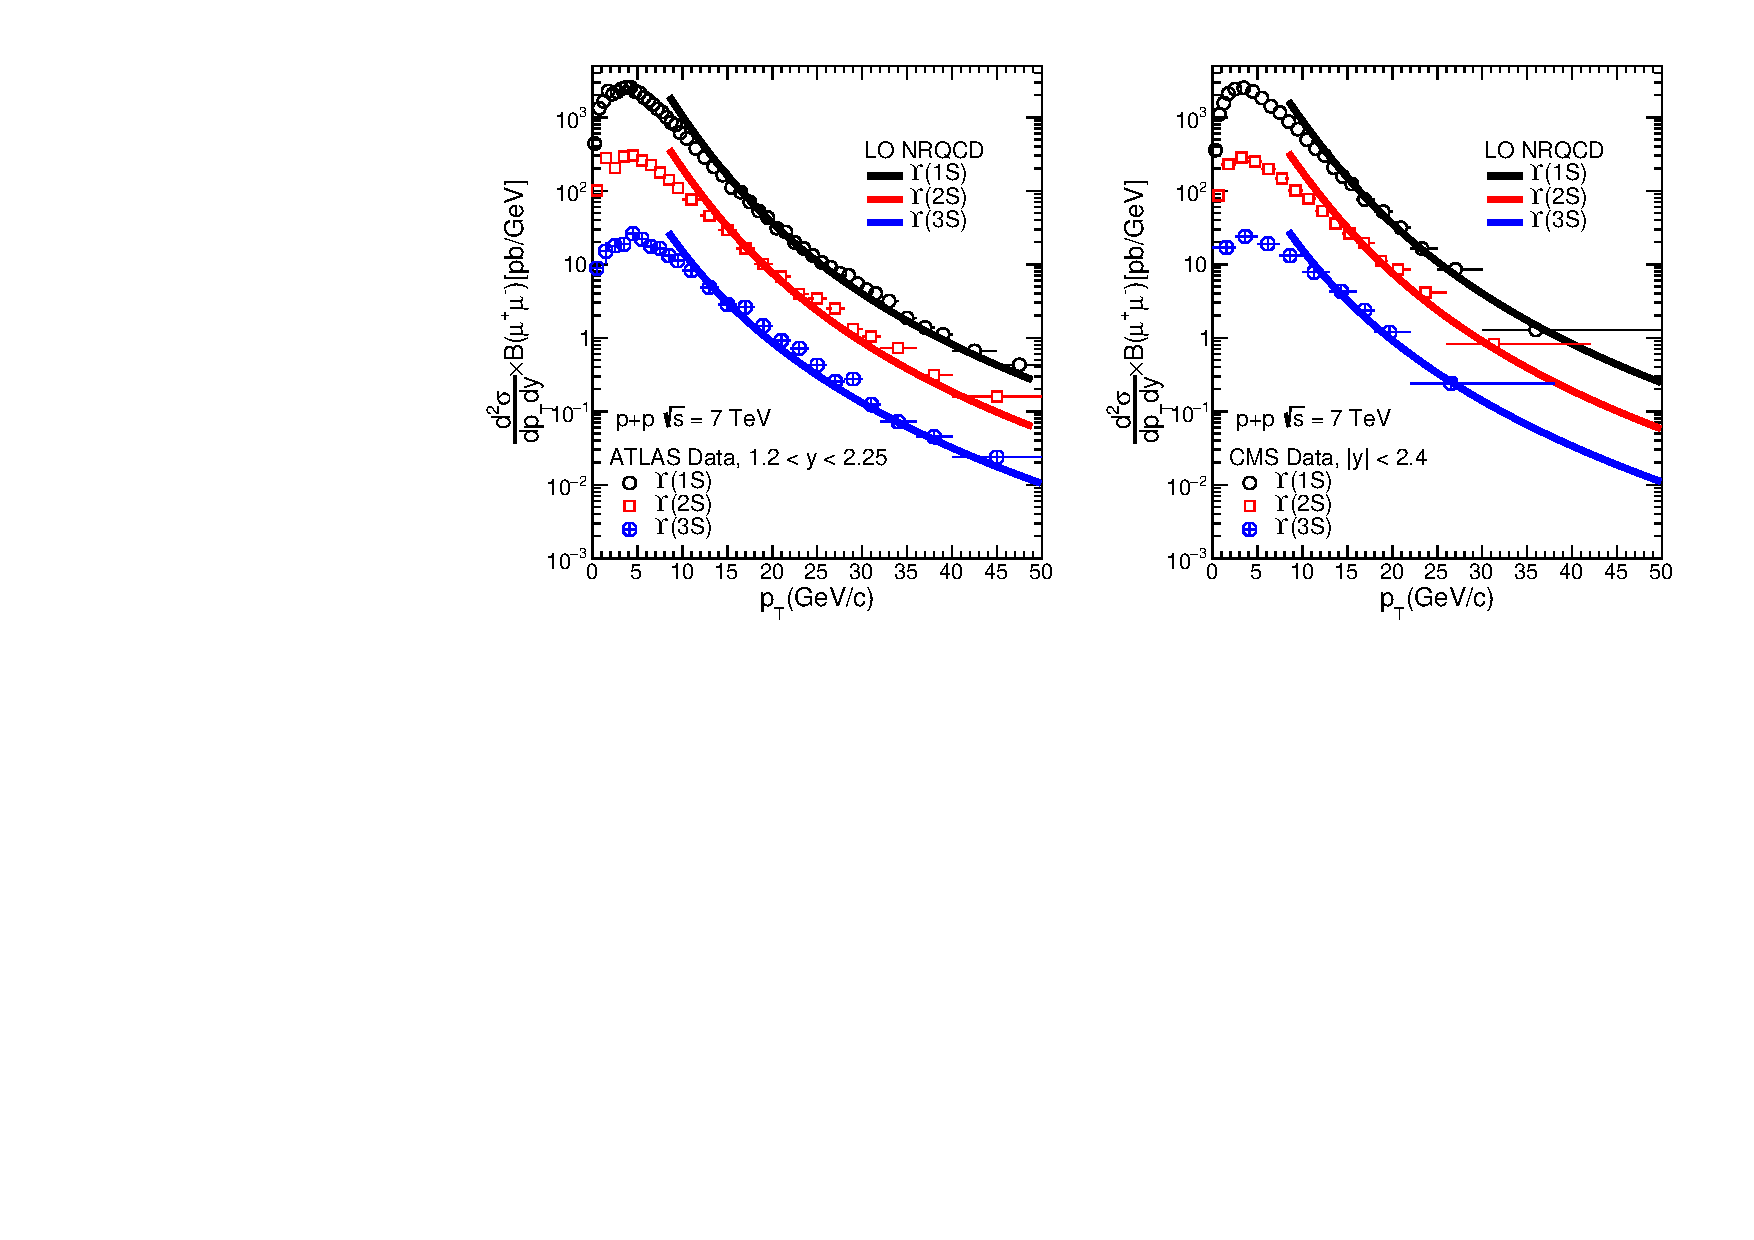
\includegraphics[width=0.99\textwidth]{Figures/Fig4_CMS_ATLAS_YnS_7TeV_Pt.pdf}
  \caption{\small{(Color online) The NRQCD calculations~\cite{Kumar:2021sek} of the production cross-section of $\Upsilon$(nS) in
      p+p collisions at $\sqrt{s}$ = 7 TeV, as a function of transverse momentum, compared with
      the measured data by ATLAS~\cite{ATLAS:2012lmu} in the left figure and CMS~\cite{CMS:2013qur}
      in the right figure. The cross-section of $\Upsilon$(1S) and $\Upsilon$(2S) as well as
      calculations are shifted vertically by factors of 10 and 5, respectively for better visibility.}}
  %   The LDMEs are obtained by a combined fit of the CMS and ATLAS data.}
  \label{Fig:SigmaYnSCMS7TeV}
\end{figure}

One requires both CS and CO matrix elements in order to get theoretical
predictions for the production of bottomonia at the Tevatron and LHC energies.
The corresponding expressions and
numerical values for CS states are obtained from Ref.~\cite{Braaten:2000cm}.
The CO states are obtained using experimentally measured data sets 
as in Refs.~\cite{Braaten:2000cm,Cho:1995vh,Cho:1995ce}. 
%The CS operators along with their theoretical values
%and the CO operators to be fitted are listed in Table~\ref{CSCO},
%where, $n$=1,2,3.
The CO elements related to p-wave states, needed as the 
feed down contributions, are obtained by Ref.~\cite{Sharma:2012dy,Feng:2015wka}.

Here we present the NRQCD results obtained in Ref.~\cite{Kumar:2021sek}.
The calculations use CT18NLO parametrisation~\cite{Hou:2019efy} for parton distribution
functions and the bottom quark mass $m_b$ is taken to be 4.88 GeV.
Measured transverse momentum distributions of $\Upsilon$(3S), 
$\Upsilon$(2S) and $\Upsilon$(1S) in p +{$\bar {\rm p}$} collisions at
$\sqrt{s}=$ 1.8 TeV and in p+p collisions at 7 TeV and 13 TeV are used to constrain
the LDMEs.

\begin{table*}
  \centering
  \caption{Comparison of CS elements and CO LDMEs extracted from fitting with experimental data
    using NRQCD formalism for $\Upsilon$(1S).}
  \footnotesize
  %\begin{tabular}{ccccccc}
  \begin{tabular*}{\textwidth}{@{\extracolsep{\fill}}lrrrrrl@{}}
    \hline
    \hline
    %& & & & & & \\
    Ref. (LO/NLO) & PDF & $m_b$ & $M_L(b\bar{b}([^3S_1]_1$ & $M_L(b\bar{b}([^3S_1]_8$ & 
    $M_L(b\bar{b}([^1S_0]_8$, & $p_T$-cut \\
    & & & $\rightarrow\Upsilon(1S)$ & $\rightarrow\Upsilon(1S)$ & $[^3P_0]_8\rightarrow\Upsilon(1S)$ & \\
    & & (GeV) & $({\rm GeV^3})$ & $({\rm GeV^3})$ & $({\rm GeV^3})$ & GeV/$c$ \\
    %& & & & & & \\
    \hline
    \hline
    & & & & & & \\
    \cite{Kumar:2021sek} (LO) & CT18 &4.88 &10.9 &0.0601$\pm$0.0017 & 0.0647$\pm$0.0016 & 8   \\
    %& (LO) & & & & & \\
    %\hline
    & & & & & & \\
    \cite{Domenech:2000ri} (LO) & CTEQ4L & 4.88 & 11.1 & 0.077$\pm$0.017 & 0 & 2 \\
    & & & & 0.087$\pm$0.016 & 0 & 4 \\
    & & & & 0.106$\pm$0.013 & 0 & 8 \\
    & & & & & & \\
    %\hline
    %& & & & & & \\
    \cite{Braaten:2000cm} (LO) & CTEQ5L & 4.77 & 12.8$\pm$1.6 & 0.116$\pm$0.027 & 0.109$\pm$0.062 & 8 \\
    & & & & 0.124$\pm$0.025 & 0.111$\pm$0.065 & \\
    & & & & & & \\
    & MRSTLO & 4.77 & 12.8$\pm$1.6 & 0.117$\pm$0.030 & 0.181$\pm$0.072 & 8 \\
    & & & & 0.130$\pm$0.028 & 0.186$\pm$0.075 & \\
    & & & & & & \\
    %\hline
    %& & & & & & \\
    \cite{Sharma:2012dy} (LO) & MSTW08LO & 4.88 & 10.9 & 0.0477$\pm$0.0334 & 0.0121$\pm$0.0400 & -  \\
    %& (LO) & & & & & \\
    %\hline
    & & & & & & \\
    \cite{Gong:2013qka} (NLO) & CTEQ6M & 4.75 & 9.282 & -0.0041$\pm$0.0024 & 0.0780$\pm$0.0043 & 8 \\
    %& (NLO) & & & & & \\
    %\hline
    & & & & & & \\
    \cite{Feng:2015wka} (NLO) & CTEQ6M & PDG & 9.282 & 0.0061$\pm$0.0024 & 0.0895$\pm$0.0248 & 8 \\
    %& (NLO) & & & & & \\
    \hline
    \hline
  \end{tabular*}
  \label{LDMEsY1S}
\end{table*}
%\normalsize

Figure~\ref{Fig:SigmaYnSCMS13TeV} shows the NRQCD calculations of production cross-section
of $\Upsilon$(nS) in p+p collisions at $\sqrt{s}$ = 13 TeV in central rapidities, as a function of
transverse momentum compared with the measured data at CMS~\cite{CMS:2017dju}
experiment. The left figure shows relative contributions in $\Upsilon$(1S) from
singlet and octet states as well as from feeddown. The right figure shows the sum
of all contributions for all the 3 states where the results for $\Upsilon$(1S) and
$\Upsilon$(2S) are shifted vertically by factors  of 10 and 5, respectively
for better visibility.


Figure~\ref{Fig:SigmaYnSCMS7TeV} shows the NRQCD calculations of the production cross-section
of $\Upsilon$(nS) in p+p collisions at $\sqrt{s}$ = 7 TeV, as a function of transverse momentum compared with
the measured data by ATLAS~\cite{ATLAS:2012lmu} in the left figure and CMS~\cite{CMS:2013qur}
in the right figure. The cross-section of $\Upsilon$(1S) and $\Upsilon$(2S) as well as
calculations are shifted vertically by factors  of 10 and 5, respectively for better visibility.

The calculations for  $\Upsilon$(3S), $\Upsilon$(2S) and $\Upsilon$(1S) are compared with 
the measured data at Tevatron and LHC~\cite{Kumar:2021sek}. The NRQCD formalism provides good description
of the data in large transverse momentum ranges at different collision energies. 
At high $p_T$, the color singlet contribution is very small and the LHC data in large $p_{\rm T}$ range 
help to constrain the relative contributions of different color octet contributions.
Table~\ref{LDMEsY1S} summarizes the LDME values for $\Upsilon$(1S) obtained by 
different groups.



\subsection{Additional methods}

In this section we, very briefly, touch upon two specialized processes namely
i) Fragmentation and ii) $k_T$ factorisation. 

\paragraph{Fragmentation}

In heavy ion collisions at high energies, the produced partons
carry large transverse momentum.
When such a parton  with large transverse momentum $(k_T)$ decays into the final
hadronic state (quarkonium state here)~\cite{frag} then the process of production is called
fragmentation. At large enough $k_T$, quarkonium production is dominated by
fragmentation instead of the short distance mechanism which 
is suppressed by powers of $m_Q/k_T$ even though fragmentation is of higher
order in $\alpha_s$~\cite{frag}. 
It was first shown by Braaten and Yuan~\cite{frag,frag1} that fragmentation of
gluons and heavy quarks
 could be an important source of large-$k_T$ quarkonia production.
 A process like $A  B \rightarrow H  X$ (where $A,B$ are  hadrons)
is factorised  into a part containing the hard-scattering cross-section which produces
 a gluon or a heavy quark 
and a part which takes care of the fragmentation of the gluon or the heavy quark into the
relevant quarkonia state. One may write 
\begin{equation}
d\sigma (A  B \rightarrow H X) = \sum_i \int_0^1 dz \ d\sigma  (A  B \rightarrow i  X) \ D_{i \rightarrow H} (x,\mu).
\end{equation}
In the above equation, $i$ is either a gluon or a heavy quark. The term $D_{i \rightarrow H} (x,\mu)$ 
is called the fragmentation function which depends on the fraction $(x)$ of momentum of the parent
parton carried by the quarkonia state and the scale $\mu$ which is of the order of $k_T$. 

 %{\bf ii) $k_T$ factorisation}
\paragraph{$k_T$ factorisation}

Another approach to quarkonium production is the $k_T$ factorisation method~\cite{kt1,kt2}.
In the  standard collinear approach, it is assumed that the momentum of all partons is
in the same direction as the initial particle and thus the  transverse momentum $(k_T)$ is
considered to be zero. But, at large collision energies, the transverse
momentum $(k_T)$ is not negligible at all. 
 
In the $k_T$ factorisation approach, the quarkonium cross section is factorised
into two parts,  a cross section ${\hat \sigma} (x, k_T, \mu)$ and a parton
density function $f(x, k_T, \mu)$, where both depend on the transverse
momentum $k_T$~\cite{kt3}.  The quarkonium cross section is given by 
 
\begin{eqnarray}
   \sigma &=& \sum_{i,j} \int \frac {dx_1}{x_1} \frac {dx_2}{x_2} \
            f_i (x_1, k_{T,1}^2, \mu) \  f_j (x_2, k_{T,2}^2, \mu) \nonumber \\
    && \times \ {\hat \sigma}_{i+j \rightarrow H} (k_{T,1}, k_{T,2}, x_1, x_2, s) \ dk^2_{T,1} \ dk^2_{T,2}.
\end{eqnarray}
where $i$ and $j$ are initial partons, $H$ is the final state,
 and ${\hat \sigma}_{i+j \rightarrow H}$ is the parton cross
section giving the probability that initial partons $i$ and $j$ will form final state $H$.
